\chapter{Features, Scenarios, and Stories}

These are the factors that drive the design of software products:
\begin{itemize}
    \item Inspiration
    \item Business/consumer needs not met by existing products
    \item Dissatisfaction with existing products
    \item Technical changes making new product types possible
\end{itemize}

We'll understand how to reach the specification of the software product we want to create. We saw that discussing requirements with the client is usually hard, mostly because of the language barrier and the fact that most clients don't even know which functionalities they want. \\

We observed that product-based software engineering requires less documentation than project-based software engineering. In Agile, requirements are not set by customers and change often. That's why developers need to identify product features: they must understand potential users and how to attract them (through interviews, surveys, informal consultations, and so on).

User representations (\textbf{personas}) and natural language descriptions (\textbf{scenarios and stories}) help identify product \textbf{features}. 

\begin{figure} [H]
    \centering
    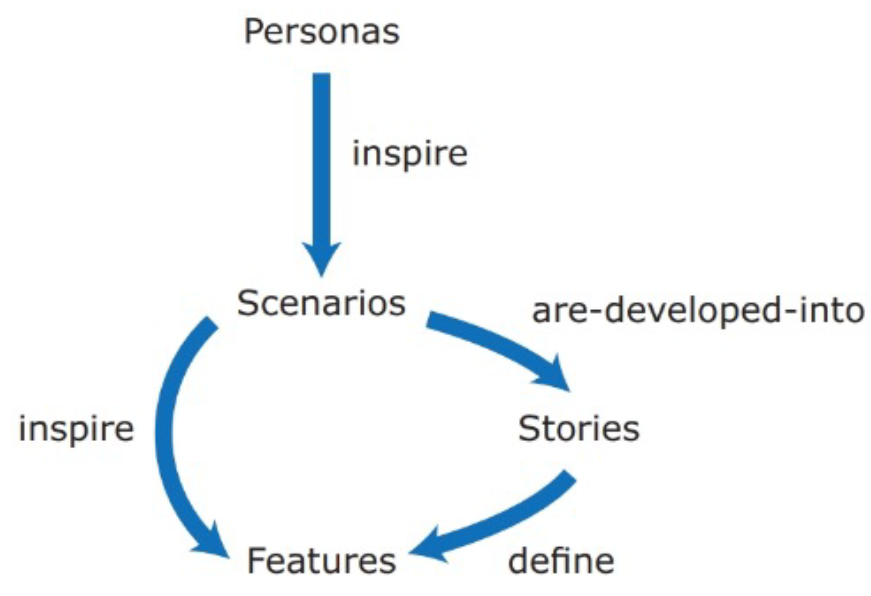
\includegraphics[width=0.48\textwidth]{images/Stories/scenariostories.png}
    \caption{Features generation process}
    \label{fig:scenariostories}
\end{figure} 

\section{Personas}

Personas are the target users for our product. Programmers need to understand potential users to design features that are useful for them. The background, skills, and experience of potential users are important because these factors will influence the user experience and the user interface. Generally, only a few (1-2, max 5) personas are required to identify key product features. Personas allow developers to “step into the users' shoes.” \\

\noindent Let's examine the key features of personas:

\begin{itemize}
    \item \textbf{Personalization}: You should give them a name and describe their personal circumstances. It is sometimes helpful to use an appropriate stock photograph to represent the person in the persona. Some studies suggest that this helps project teams use personas more effectively.
    \item \textbf{Job-related}: If your product is targeted at businesses, you should describe their job and (if necessary) what the job involves. For some jobs, such as teaching, where readers are likely familiar with the role, this may not be necessary.
    \item \textbf{Relevance}: If possible, you should explain why they might be interested in using the product and what they might want to do with it.
    \item \textbf{Education}: You should describe their educational background and their level of technical skills and experience. This is important, especially for interface design.
\end{itemize}

\begin{figure} [H]
    \centering
    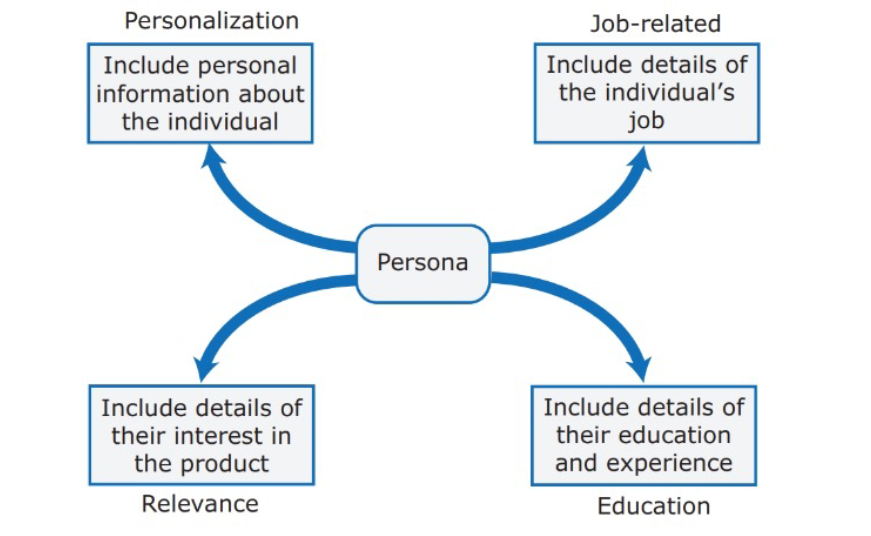
\includegraphics[width=0.8\textwidth]{images/Stories/personadescription.png}
    \caption{Personas' key features}
    \label{fig:personadescription}
\end{figure} 

Some developers also use an appropriate stock photograph to represent the person in the persona. Studies have shown that we have biases depending on the photo, so not everyone accepts the use of pictures. When studying users is not possible (e.g., for some new products), we can develop proto-personas: these are imagined personas.

\section{Scenarios}

Once the personas are created, the next step is to work with scenarios. To discover product features, we can define \textbf{scenarios} of user interactions with the product. A scenario is a narrative describing a situation in which a user is using our product’s features to accomplish a specific goal. \\

Let's examine the key features of scenarios:

\begin{figure} [H]
    \centering
    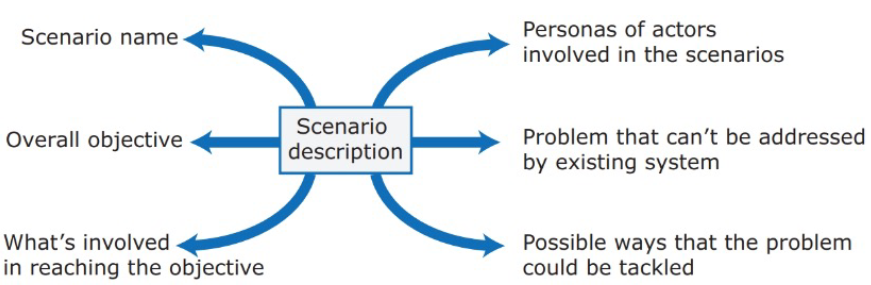
\includegraphics[width=0.8\textwidth]{images/Stories/scenariodescription.png}
    \caption{Scenario's key features}
    \label{fig:scenariodescription}
\end{figure} 

Narrative, high-level scenarios facilitate communication and stimulate design creativity. Scenarios are not specifications, though; they lack details and may be incomplete. Usually, several scenarios (e.g., 3-4) are required for each persona, covering the main responsibilities of the persona. The scenarios are written from the \emph{user’s perspective}. Each team member should individually create some scenarios, then discuss them with the rest of the team and, if possible, with users.

\section{User Stories}

Scenarios are high-level stories of product use, while user stories are finer-grained narratives. They follow a structure, which is as follows: 

As a \textit{<role>} I want to \textit{<do something>} so that \textit{<reason/values>}.

\newpage

User stories are not part of the Agile manifesto, but they help to adhere to Agile principles: 
\newline \noindent - Our highest priority is to satisfy the customer through early and continuous delivery of valuable software.
\newline \noindent - Working software is the primary measure of progress.
\newline \noindent - Simplicity, the art of maximizing the amount of work not done, is essential. \\

User stories also help visualize the progress made in our program. We can write the short stories on sticky notes to stick them on a to-do board. We need to remember that \emph{stories that don't create business value for the customer are work that isn't going to count as progress. Additionally, creating stories that depend on one another might create deadlocks}. \\

The Scrum product backlog is often a set of user stories. Long stories (\emph{epics}) must be broken into simpler stories. Stories are associated with \textbf{priorities} (and possibly also with an estimate of effort needed to implement the story) and sorted according to priority (\emph{requirements triage}). It is possible to express all the functionalities described in a scenario as user stories, but scenarios read more naturally, making it easier to understand stories and providing more context (we can sell stories to stakeholders).

The final goal of the user stories is to identify the features that define our product. These features should, in principle, have the following properties:

\begin{itemize}
    \item \textbf{Independence}: A feature should not depend on how other system features are implemented and should not be affected by the order of activation of other features.
    \item \textbf{Coherence}: Features should be linked to a single item of functionality. They should not do more than one thing and should never have side effects.
    \item \textbf{Relevance}: System features should reflect the way users normally carry out some tasks. They should not offer obscure functionality that is rarely required.
\end{itemize}
\newpage
The knowledge required for feature design is:

\begin{figure} [H]
    \centering
    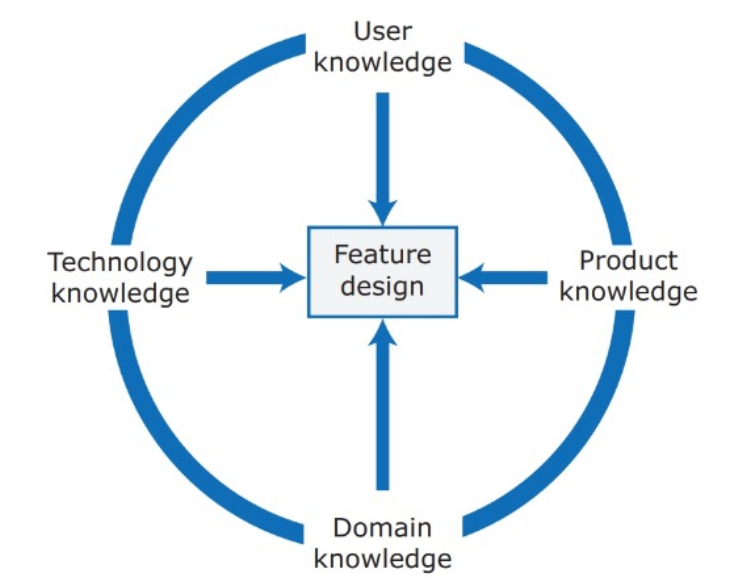
\includegraphics[width=0.6\textwidth]{images/Stories/feature_design.png}
    \caption{Feature design knowledge required}
    \label{fig:featuredesign}
\end{figure} 

\begin{itemize}
    \item \textbf{User Knowledge}: You can use user scenarios and user stories to inform the team of what users want and how they might use the software features.
    \item \textbf{Product Knowledge}: You may have experience with existing products or decide to research what these products do as part of your development process. Sometimes your features have to replicate existing features in these products because they provide fundamental functionality that is always required.
    \item \textbf{Domain Knowledge}: This is knowledge of the domain or work area (e.g., finance, event booking) that your product aims to support. By understanding the domain, you can think of new innovative ways of helping users accomplish their goals.
    \item \textbf{Technology Knowledge}: New products often emerge to take advantage of technological developments since their competitors were launched. If you understand the latest technology, you can design features to make use of it.
\end{itemize}

\newpage
It's important to find a balance between opposing factors in feature design.

\begin{figure} [H]
    \centering
    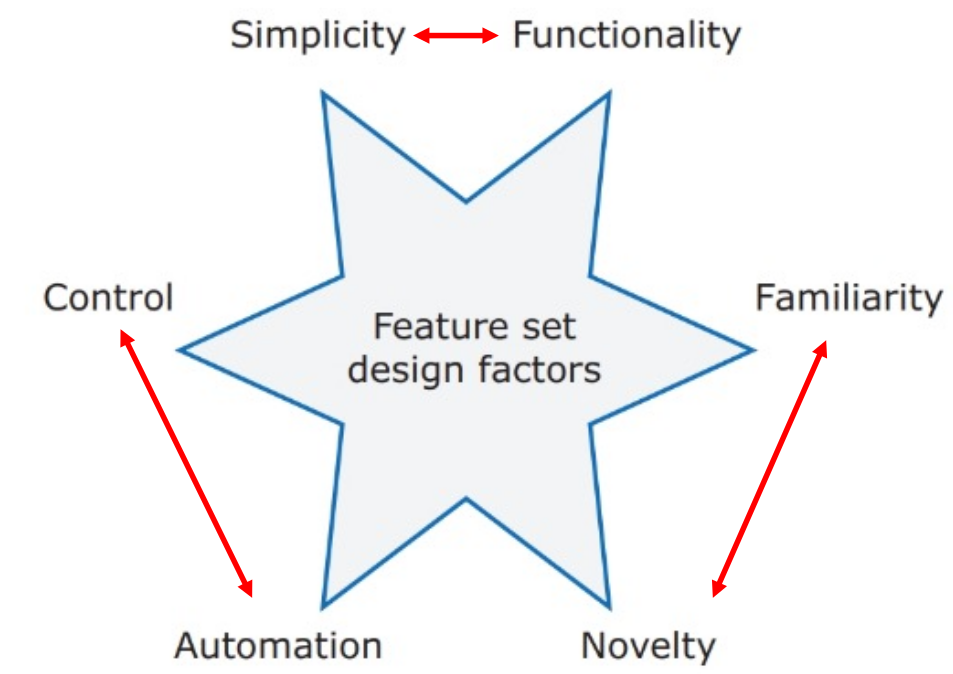
\includegraphics[width=0.6\textwidth]{images/Stories/factors_design.png}
    \caption{Factors in feature design}
    \label{fig:factorsdesign}
\end{figure}

The number of product features grows as new potential users are envisaged (this is also known as \textbf{Feature Creep}). This growth is dictated by marketing executives who want to meet all users' demands. Marketing also pressures teams to include competitors' features and has the desire to support both experienced and inexperienced users. To avoid feature creep, making feature questions usually allows understanding which features are pointless.

\begin{figure} [H]
    \centering
    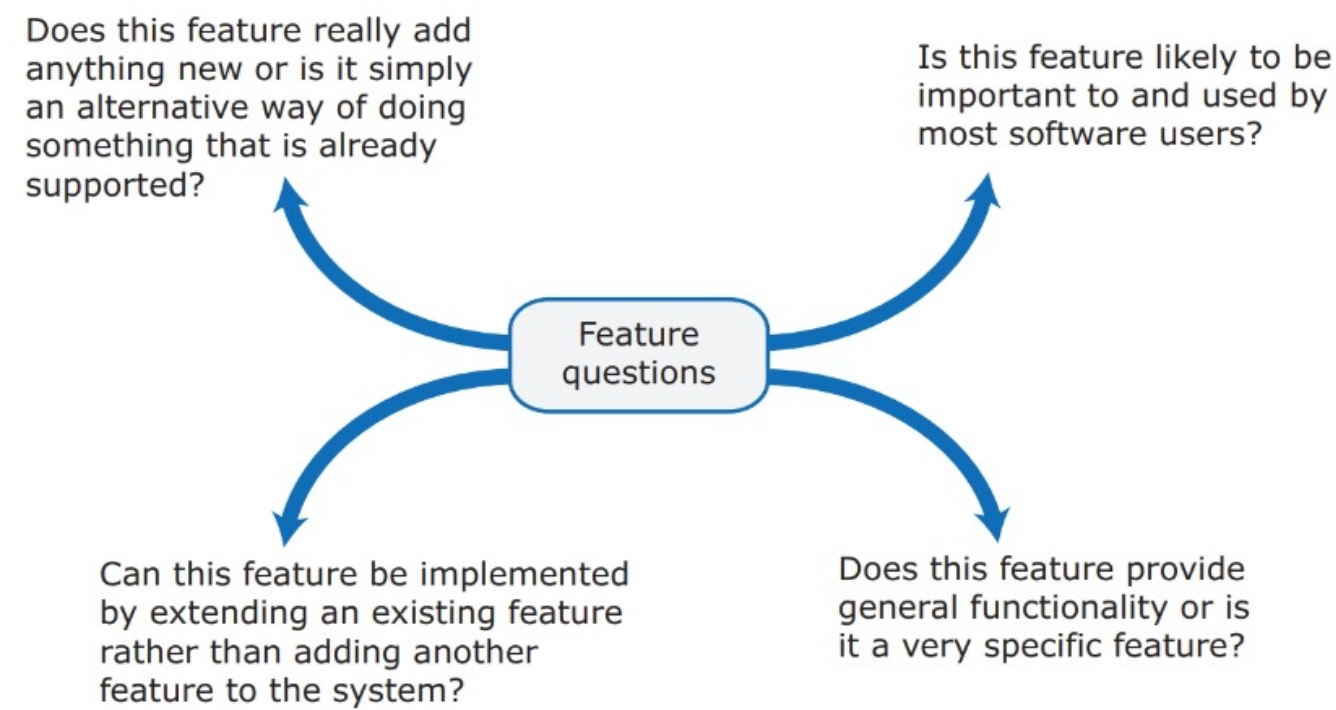
\includegraphics[width=0.9\textwidth]{images/Stories/feature_creep.png}
    \caption{Feature questions to avoid feature creep}
    \label{fig:featurecreep}
\end{figure}
\newpage

The product development team must meet to discuss scenarios and stories to extract the list of product feature descriptions. This consists of detecting the input and activation for the action required in the feature and then writing the expected output for the action.

\begin{figure} [H]
    \centering
    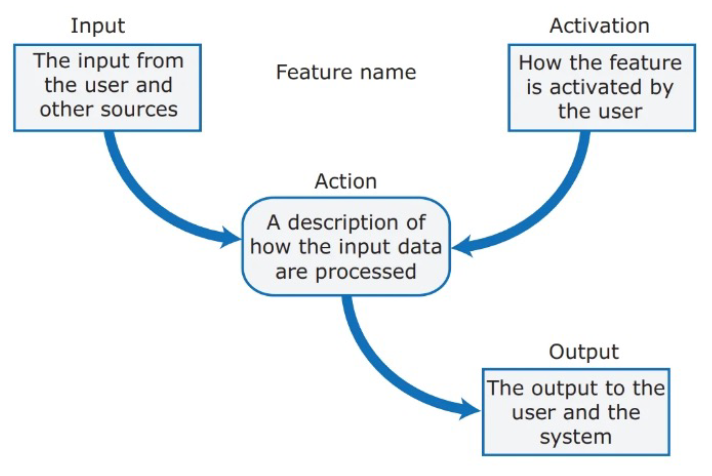
\includegraphics[width=0.8\textwidth]{images/Stories/Feature_derivation.png}
    \caption{Feature derivation}
    \label{fig:featurederivation}
\end{figure}
